\section{Requirement Analysis}

This section presents a comprehensive analysis of the functional and non-functional requirements derived from stakeholder needs. The requirements engineering process followed a structured elicitation pipeline, initiating with qualitative interviews with four primary faculty stakeholders: Aloke Sir, Shafiq Sir, Plabon Sir, and Bilkis Ma'am. The qualitative data was processed via thematic analysis to resolve explicit architectural trade-offs, concluding with the formal specification and validation of system attributes.

\subsection{Stakeholders}
To map the operational boundaries of the proposed framework, structured interviews were conducted to identify architectural tensions. The feedback highlighted three critical constraints that the underlying system design reconciles:

\begin{enumerate}
    \item \textbf{The Update Paradox:} While a strictly offline, air-gapped environment satisfies the mandate for exam data isolation, it risks system obsolescence. Our architecture resolves this through a \textbf{Federated Learning (FL) Layer}, allowing for encrypted model weight updates without exposing raw data to external servers.
    \item \textbf{The Capability-Resource Gap:} To bridge the gap between cloud-level intelligence and institutional hardware, the system utilizes a quantized \textbf{Qwen2.5-1.5B-Instruct} model, optimized for local CPU execution within 8GB RAM constraints.
    \item \textbf{The Mixed-Mode Access Friction:} Academic integrity is maintained via \textbf{LoRA Adapter modules}, ensuring the shared core model applies role-specific logic, keeping public learning materials and protected assessment artifacts in logically distinct, cryptographically isolated pathways.
\end{enumerate}

The refined operational mandates for the system actors are defined below:

\begin{itemize}
    \item \textbf{Students:} Interact with the RAG pipeline to query public educational materials. The runtime is strictly restricted by an \textbf{Output Privacy Guard} that prevents the model from reconstructing protected assessment artifacts, ensuring grounded study support.
    \item \textbf{Teachers:} Utilize the \textbf{Bloom Taxonomy Review Module} for cognitive moderation. This role requires intra-departmental cryptographic isolation, ensuring active exam drafts remain invisible to peers, while providing automated access to cognitive-tier classification (6 levels) and higher-order question rewrites.
\end{itemize}

\subsection{Functional Requirements}
Functional requirements define the core behaviors and actions the academic assistant must execute. 

\begin{small}
\begin{longtable}{|p{0.09\textwidth}|p{0.17\textwidth}|p{0.52\textwidth}|p{0.14\textwidth}|}
\caption{System Functional Requirements Specification} \label{tab:functional_requirements} \\
\hline
\textbf{ID} & \textbf{Component} & \textbf{Description} & \textbf{Trace.} \\ \hline
\endhead
FR-1 & Role-Aware LoRA & Load LoRA adapters per role: student RAG vs.\ teacher Bloom classification. & App.~A \\ \hline
FR-2 & Federated Aggregation & Encrypted local adapter updates; server FedAvg without raw text. & App.~A \\ \hline
FR-3 & Output Privacy Guard & Post-filter student outputs to block protected exam leakage. & App.~A \\ \hline
FR-4 & Bloom Tiering & Six Bloom levels plus reason and higher-order rewrite for teachers. & App.~A \\ \hline
FR-5 & Multi-Modal Ingestion & PDF, image, text via PyMuPDF and Tesseract with metadata. & App.~A \\ \hline
FR-6 & Corpus Isolation & Separate public vs.\ protected FAISS indexes by access level. & App.~A \\ \hline
\end{longtable}
\end{small}

\subsection{Non-Functional Requirements}
Non-functional requirements define the security boundaries and operational constraints.

\begin{small}
\begin{longtable}{|p{0.09\textwidth}|p{0.17\textwidth}|p{0.52\textwidth}|p{0.14\textwidth}|}
\caption{System Non-Functional Requirements Specification} \label{tab:non_functional_requirements} \\
\hline
\textbf{ID} & \textbf{Attribute} & \textbf{Description} & \textbf{Trace.} \\ \hline
\endhead
NFR-1 & On-premises & No mandatory cloud LLM API; local GGUF and FAISS. & App.~A \\ \hline
NFR-2 & Resource limits & CPU GGUF inference; $\approx$1\,GB model file; 8\,GB RAM target. & App.~A \\ \hline
NFR-3 & Role isolation & Public vs.\ protected retrieval boundaries. & App.~A \\ \hline
NFR-4 & Maintainability & Modular Python packages and version-pinned deps. & App.~A \\ \hline
NFR-5 & Human-in-the-loop & Teacher review required for moderation outputs. & App.~A \\ \hline
\end{longtable}
\end{small}

\section{System Overview / Architecture}

The proposed Privacy-Preserving Education AI framework utilizes a dual-pipeline architecture to support distinct academic roles—students and teachers—while maintaining strict data localization and security. The system operates entirely on-premises, relying on a quantized Qwen2.5-1.5B-Instruct model to provide efficient, CPU-only inference. The system is organized into six major functional components: Document Ingestion and Parsing, Metadata-Aware Vector Knowledge Base, Role-Aware RAG and Moderation Pipelines, Shared Local LLM Core, Output Privacy Guard, and the Federated Learning Layer. Figure~\ref{fig:system_architecture_report} presents the high-level system architecture.

\begin{figure}[H]
    \centering
    
\includegraphics[width=0.95\textwidth]{images/final.jpeg}
    \caption{Role-separated system architecture for privacy-constrained academic assistance.}
    \label{fig:system_architecture_report}
\end{figure}

\subsection{High-Level Architecture}

The ingestion layer receives documents from teachers or students. Public learning materials are routed to the public vector store. Protected assessment artifacts are routed to the protected vector store and teacher-only moderation workflow. Student queries are answered using public retrieval only. If a student prompt or generated answer appears to reconstruct protected material, the privacy guard blocks the response or routes the user toward safe study alternatives.

Teacher queries can access protected artifacts for moderation. This design preserves legitimate teacher use while preventing students from retrieving confidential exam content.
          \begin{figure}[H]
        \centering
        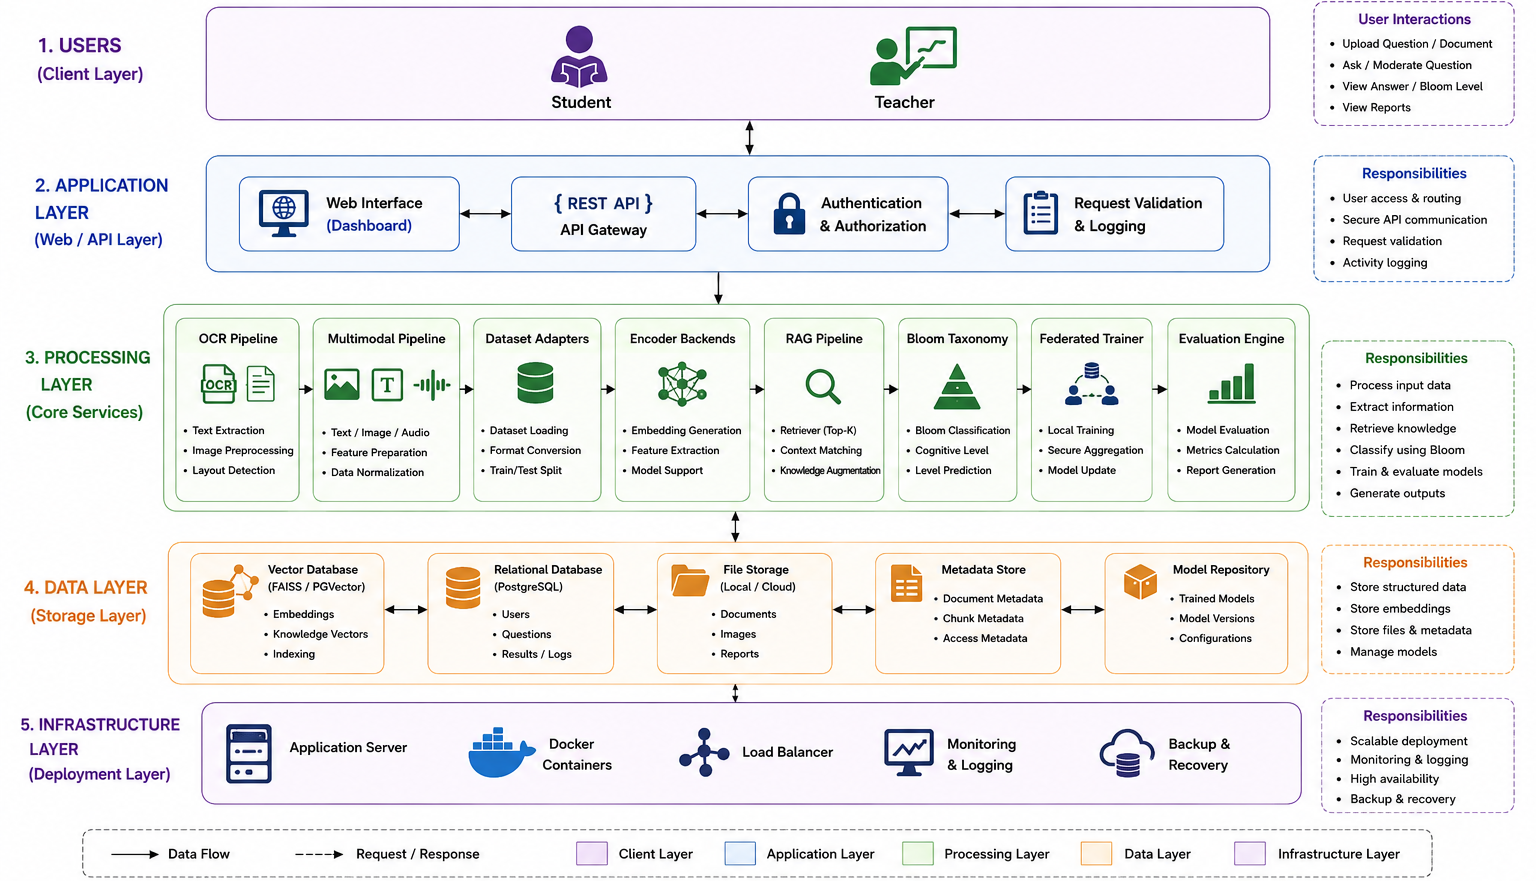
\includegraphics[width=0.9\textwidth]{images/hightlevelarch.png} % 
        \caption{High-Level Architecture}
        \label{fig:system_architecture}
    \end{figure}

\subsection{Detailed Design Diagrams}
To provide a comprehensive understanding of the system's operational mechanisms, data movement, and structural interactions, the system design is visualized through standard engineering representations. These diagrams clarify the modular communication, logical sequence of operations, and the data lifecycle within the privacy-preserving framework.

\begin{itemize}
    \item \textbf{Block Diagram:} Figure \ref{fig:system_architecture} illustrates the high-level architecture, showcasing functional modules such as multi-modal document ingestion, metadata-aware parsing, and the role-specific RAG/Moderation pipelines. This diagram highlights the convergence of student and teacher workflows into the shared \textbf{Qwen2.5-1.5B} local core.
    
    \begin{figure}[H]
        \centering
        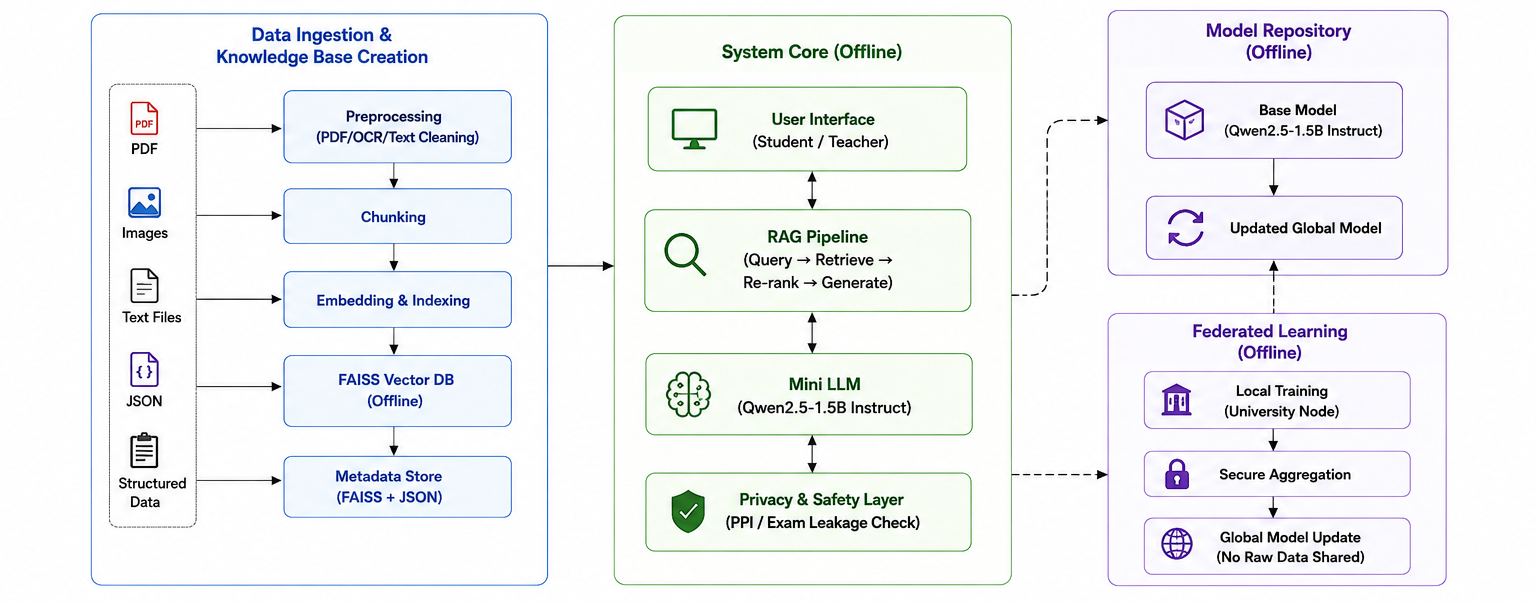
\includegraphics[width=0.9\textwidth]{images/blockdiagram.png} % Replace with your image filename
        \caption{Block Diagram}
        \label{fig:system_architecture}
    \end{figure}

    \item \textbf{Data Flow Diagram (DFD):} This representation maps the transition of multi-modal data (PDF, Image, Text) from the initial input phase, through the OCR and text-cleaning stages, into the \textbf{FAISS Vector Database}. It explicitly demonstrates how data remains localized and encrypted throughout the processing loop.
    \begin{figure}[H]
        \centering
        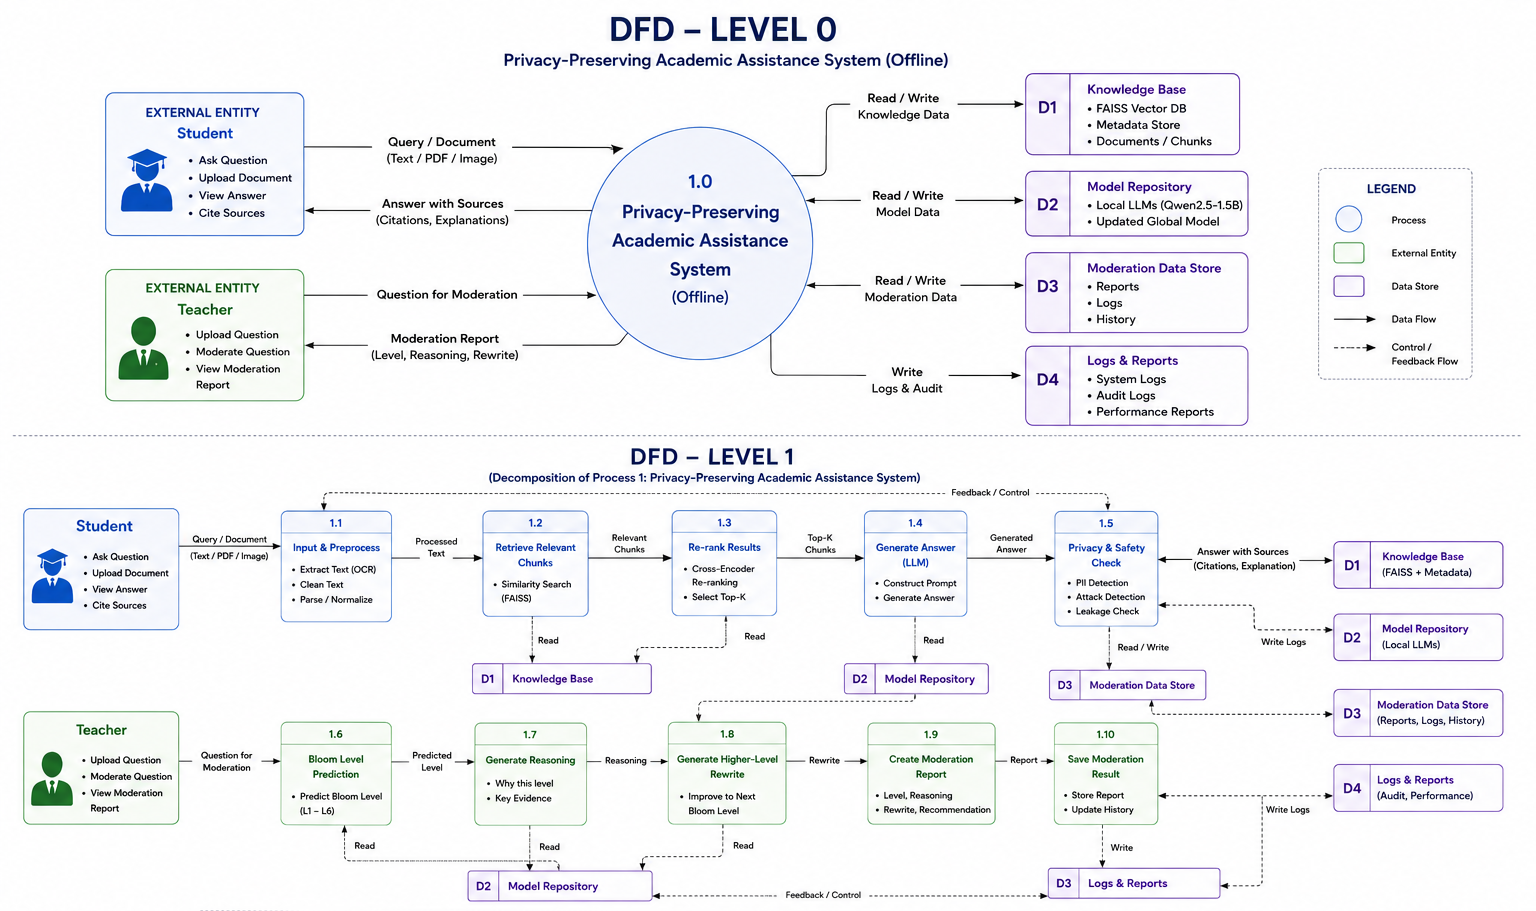
\includegraphics[width=0.9\textwidth]{images/dfd.png} % 
        \caption{Data Flow Diagram (DFD) Level 1}
        \label{fig:system_architecture}
    \end{figure}
    \item \textbf{Flowchart (Logic Sequence):} The flowchart depicts the logical algorithm followed by the system when a user submits a query. It captures the decision gate (Student vs. Teacher), the \textbf{LoRA adapter} selection, and the conditional flow between the grounded RAG engine and the \textbf{Bloom Taxonomy Moderation} module.
         \begin{figure}[H]
        \centering
        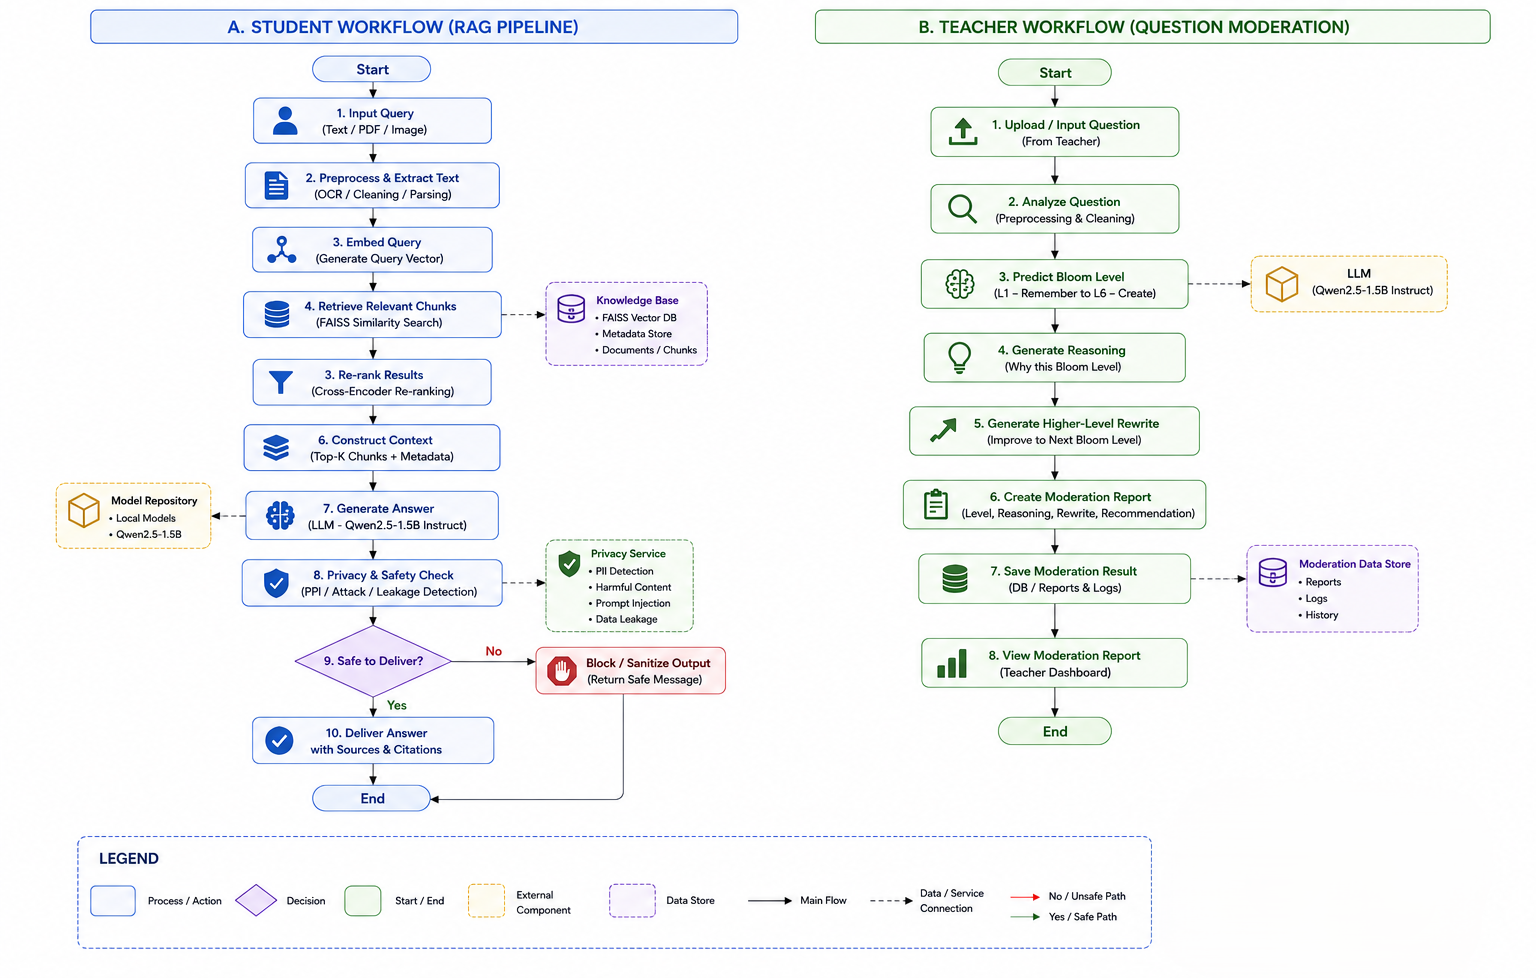
\includegraphics[width=0.9\textwidth]{images/flowchart.png} % 
        \caption{Flowchart}
        \label{fig:system_architecture}
    \end{figure}

    \item \textbf{UML Diagrams:} These standardized visualizations provide a dual view of the system: the Class Diagram defines the static architecture, mapping the relationships between the shared Qwen2.5-1.5B core, role-specific LoRAAdapters, and the KnowledgeBase entities; simultaneously, the Sequence and Activity Diagrams delineate the dynamic behavioral logic, tracing the chronological data flow of student queries and the conditional decision gates within the teacher-led moderation pipeline to ensure all privacy-preserving constraints are programmatically enforced.
              \begin{figure}[H]
        \centering
        
\includegraphics[width=0.9\textwidth]{images/uml.jpg} % 
        \caption{UML DiagramS(Class, Sequence, Activity)}
        \label{fig:system_architecture}
    \end{figure}

    \item \textbf{Database Design / ER Diagram:} This diagram defines the schema for the \textbf{Metadata-Aware Repository}. It illustrates how entity attributes such as \texttt{access\_level}, \texttt{source}, \texttt{page\_number}, and \texttt{modality} are stored to ensure strict separation between public learning assets and protected assessment artifacts.
         \begin{figure}[H]
        \centering
        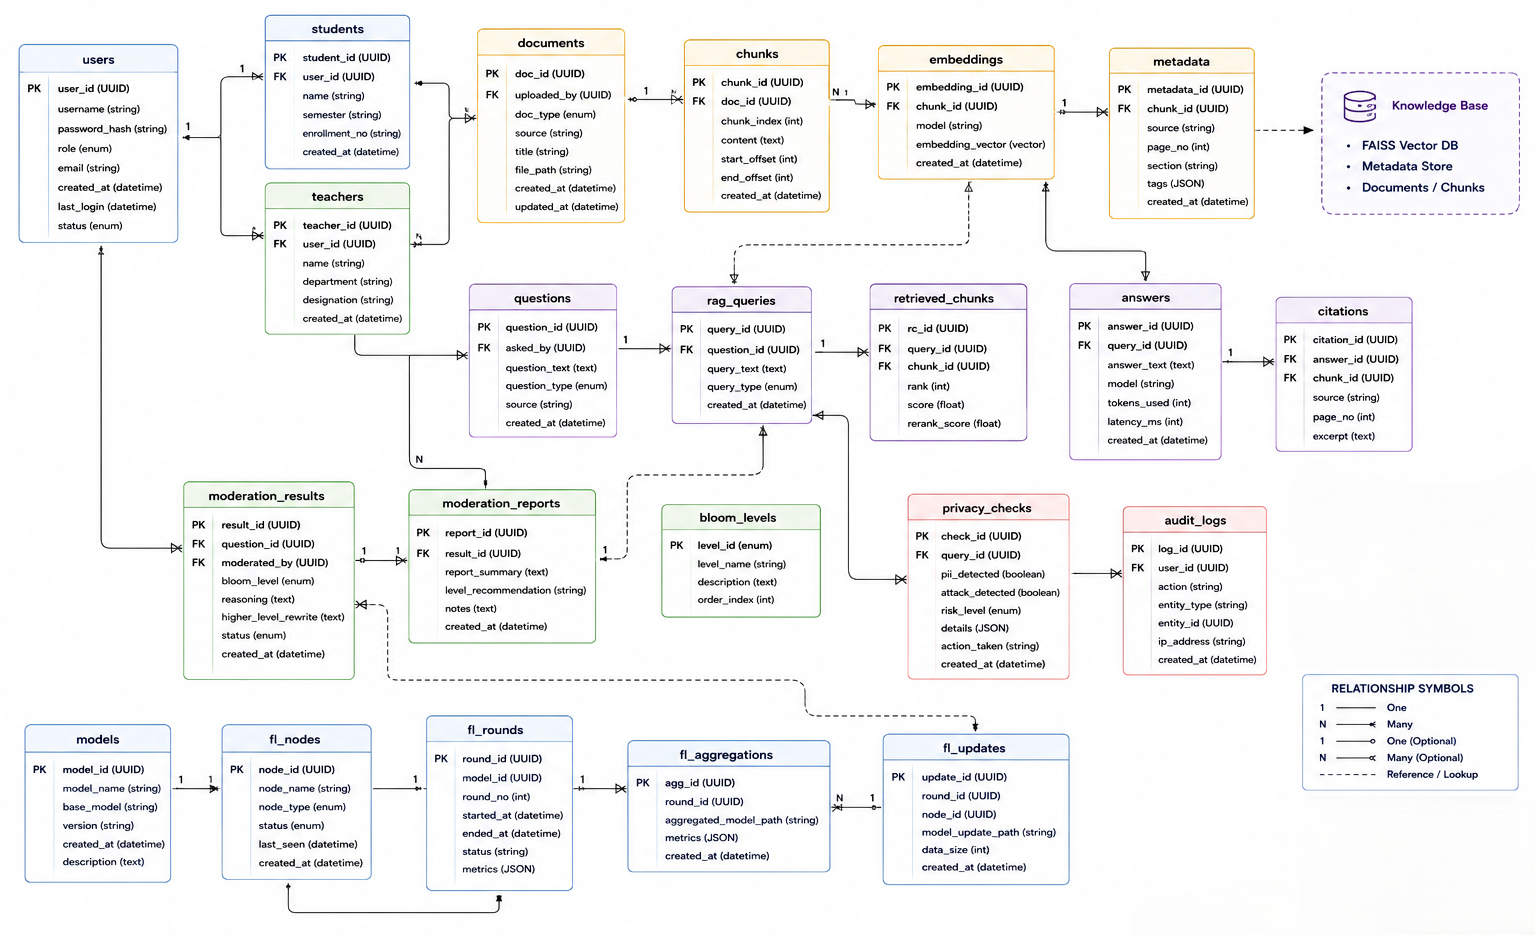
\includegraphics[width=0.9\textwidth]{images/er.png} % 
        \caption{Database Design / ER Diagram}
        \label{fig:system_architecture}
    \end{figure}
\end{itemize}

\section{Design Alternatives and Rationale}

Several alternatives were considered:
\begin{itemize}
    \item \textbf{Single shared corpus:} simple to implement but unsafe because protected exam content could be retrieved for students.
    \item \textbf{Cloud LLM service:} powerful but may expose course documents externally and increase operating cost.
    \item \textbf{Local role-separated RAG:} slightly more complex but better aligned with assessment confidentiality and local deployment.
    \item \textbf{Formal differential privacy:} stronger theoretical privacy, but not implemented in the current prototype and therefore not claimed.
\end{itemize}

The selected design is local role-separated RAG with metadata preservation and privacy screening. This choice balances student utility, teacher moderation needs, privacy constraints, and resource limits.

\section{Algorithmic Flow / Pseudocode}

\begin{algorithm}[H]
\caption{Student-facing guarded RAG workflow}
\begin{algorithmic}[1]
\Require User query $q$, role $r$, public store $P$, protected store $S$
\If{$r$ is teacher}
    \State Retrieve from authorized store according to teacher workflow.
    \State Return moderation or Bloom-support output.
\Else
    \If{PrivacyGuard detects reconstruction intent in $q$}
        \State Return safe refusal and suggest public study alternative.
    \EndIf
    \State Retrieve top public chunks from $P$.
    \State Generate answer from retrieved public context.
    \If{PrivacyGuard detects protected reconstruction in answer}
        \State Suppress answer and return safe alternative.
    \Else
        \State Return grounded answer with public evidence.
    \EndIf
\EndIf
\end{algorithmic}
\end{algorithm}

\section{Summary}

This chapter presented the requirements, architecture, module design, and algorithmic flow of the system. The design emphasizes public/protected separation, local operation, metadata preservation, and conservative privacy screening. The next chapter describes how the system was implemented and evaluated.
